\chapter{Introduction}

Scientists, engineers, and researchers use wireless sensor networks (WSN) for a wide array of applications. Many of these applications rely on knowledge on the precise position of each node. While some may only require relative coordinates within the network, most biological, geophysical, and other scientific applications require coordinates on a global coordinate system. Perhaps the obvious solution is for each node in the network to be equipped with GPS or other location positioning service.  However, constraints on cost, power consumption, as well as visibility of satellites forbids this.  

Many protocols have been propopsed\cite{DV-HOP,MDS-MAP,CCA-MAP07} to calculate relative positions amongst the nodes of a network.  They vary in the required network functionality in terms of radio ranging or range-free.  However, in all cases, in order to convert from relative to global coordinates, some of the nodes do require a local source of global coordinates by using GPS or some other source.  This can be achieved by operators recording the global coordinates during network deployment or by the device having GPS embedded in a subset of the nodes.  We call these enhanced nodes anchors.  Here, we explore the effect of anchor node placement within the network on the overall localization errors, on a network-wide basis. This provides network planners with a set of general rules to minimize the number of anchor nodes required while avoiding poor node localization, allowing scientists to assume a maximum position error during their own research.

\section{Motivation} 
During previous work designing localization protocols\cite[p. 11]{CCA-MAP09}, authors often choose anchors at random within the network.  Frequently, their simulations are run multiple times with different anchors in order to statistically exclude anchor node placement from their results. Figure [TODO] demonstrates this using a CCA simulation.  This phenomenon led to this quest to determine the best anchor node placement.

//TODO Include result plot showing varying errors for same network with different anchors

In practical applications, scientists and engineers do not have the luxury of running their localization protocols multiple times to detemine the best location.  In fact, this would defeat the purpose of the localalization protocol in the first place.  Therefore, it is critical to be able to assign a maximum location error to all the nodes in a network so that data processing that relies on location can effectively take the location error into account.  

\section{Thesis Contribution}
We demonstrate that by avoiding certain poor anchor node placements, extremely poor location errors can be avoided.  Further, we demonstrate that other than these edge cases, the location error falls within a statistically insignificant range, where the range can be determined based on network connectivity and topology.  Specifically, we show that the propability of extremely high location error result from anchor nodes being roughly in a geographically straight line.  As the anchor nodes are spread out from a straigh line, the propability of high errors decreases, leaving network designers a relatively simple chore when choosing anchor nodes locations.

\section{Methodology}
Many localization protocols and algorithms provide a set of relative coordinates that are then transformed into global coordinates.  For the purpose of this research, we chose CCA-MAP\cite{CCA-MAP07,CCA-MAP09} as the algorithm to provide simulation results.  A Matlab\copyright  simulation of this algorithm already existed from Li Li\cite{CCA-MAP07}, and was modified to provide the necessary output statistics presented here.  CCA-MAP is described in more detail in \ref{sec:CCA-MAP} on page \pageref{sec:CCA-MAP}.

\section{Thesis Organization}
A brief background of Wireless Sensor Networks and localization protocols in general are presented in Chapter 2.  Chapter 3 presents the limited related work in anchor node placement, in particular.  Chapter 4 contains the various anchor node placements and summaries of how they perform.  The cause of the extreme edge cases comes to light in Chapter 5, along with a discussion of the Procrustes algorithm.  Chapter 6 presents conclusions and future work.

%\begin{figure} % % Requires \usepackage{graphicx} % \centering %
%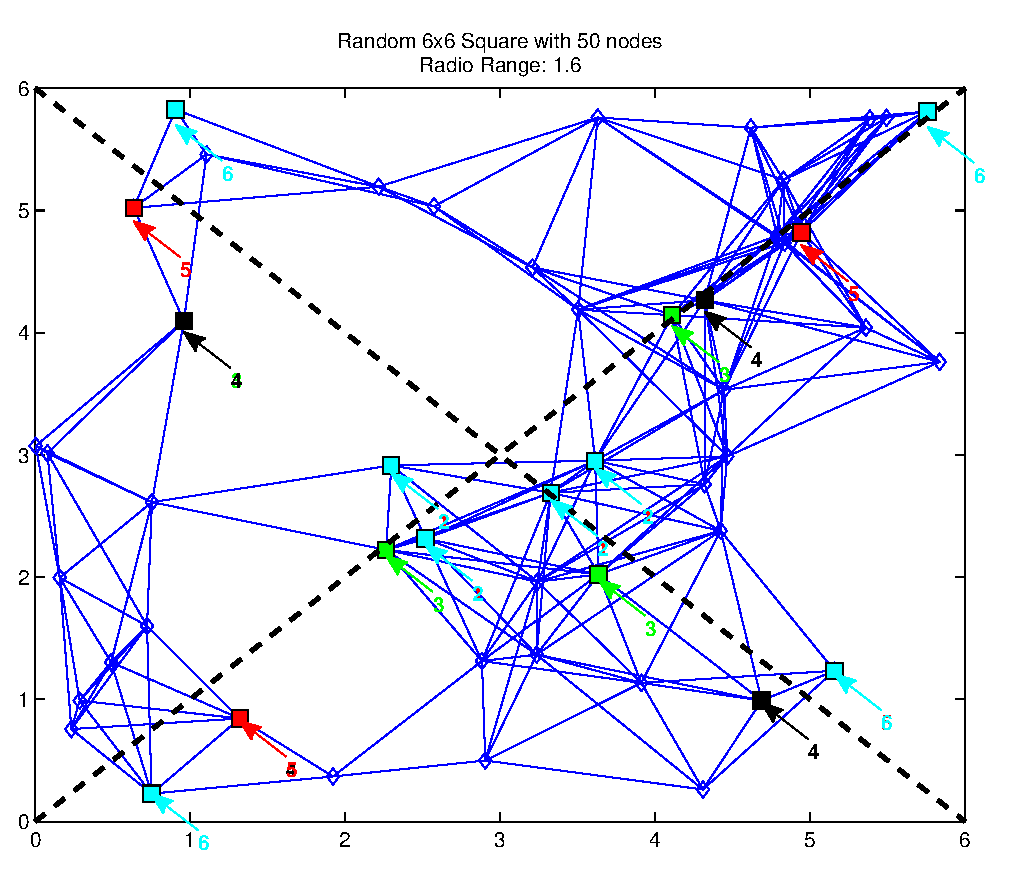
\includegraphics[width=4in]{../cca/results/45DegreeAxis_Random/networkRandom6x6Squarewith50nodes1-6Radius.eps}\\
% \caption{The random network used, showing the 6 position sets of anchors.} %
%\label{fig:45DegreeAxisRandomNetwork} %\end{figure}

%\begin{equation}\label{eqn:newton_law} %    F = Ma %\end{equation}
%Paragraph referencing an equation \ref{eqn:newton_law}.
